\documentclass[../open-optimization/open-optimization.tex]{subfiles}

\begin{document}

\chapter{Exponential Size Integer Programming Formulations}
\label{sec:exponential-IP-forumulations}

Although typically models need to be a reasonable size in order for us to code them and send them to a solver, there are some ways that we can allow having models of exponential size.  The first example here is the cutting stock problem, where we will model with exponentially many variables.  The second example is the traveling salesman problem, where we will model with exponentially many constraints.  We will also look at some other models for the traveling salesman problem.  
\section{Cutting Stock}
This is a classic problem that works excellent for a technique called \emph{column generation}.
We will discuss two versions of the model and then show how we can use column generation to solve the second version more efficiently.  First, let's describe the problem.

\begin{general}{Cutting Stock}{}
You run a company that sells of pipes of different lengths.  These lengths are $L_1, \dots, L_k$.  To produce these pipes, you have one machine that produces pipes of length $L$, and then cuts them into a collection of shorter pipes as needed.  

You have an order come in for $d_i$ pipes of length $i$ for $i=1, \dots, k$.  How can you fill the order while cutting up the fewest number of pipes?
\end{general}
\begin{example}
A plumber stocks standard lengths of pipe, all of length 19 m. An order arrives for:
\begin{itemize}
\item  12 lengths of 4m
\item 15 lengths of 5m
\item 22 lengths of 6m
\end{itemize}
How should these lengths be cut from standard stock pipes so as to minimize
the number of standard pipes used?
\end{example}
\begin{center}
%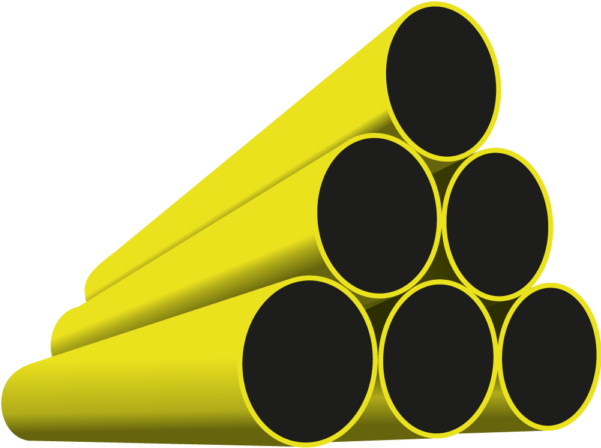
\includegraphics[scale = 0.1]{pipes}
%https://www.freeimages.com/search/sawing-pipe
\end{center}

An initial model for this problem could be constructed as follows:  
\begin{itemize}
\item Let $N$ be an upper bound on the number of pipes that we may need.
\item Let $z_j = 1$ if we use pipe $i$ and $z_j = 0$ if we do not use pipe $j$, for $j=1, \dots, N$.
\item Let $x_{ij}$ be the number of cuts of length $L_i$ in pipe $j$ that we use.
\end{itemize}
Then we have the following model
\begin{equation}
\begin{split}
\min\ \  & \sum_{j=1}^N z_j\\
\st \ \  & \sum_{i=1}^k  L_i x_{ij} \leq Lz_j \ \text{ for } j=1,\dots, N\\
& \sum_{j=1}^N x_{ij} \geq d_i \ \text{ for } i=1, \dots, k\\
& z_j \in \{0,1\} \text{ for } j=1, \dots, N\\
& x_{ij} \in \Z_+ \text{ for } i=1, \dots, k,\, j=1, \dots, N
\end{split}
\end{equation}
\begin{exercise}
In the example above, show that we can choose $N=16$.
\end{exercise}
For our example above, using $N=16$, we have
\begin{equation}
\begin{split}
\min\ \  & \sum_{j=1}^{16} z_j\\
\st \ \  &  4 x_{1j} + 5 x_{2j} + 6 x_{3j} \leq 19 z_j\\
& \sum_{j=1}^{16} x_{1j} \geq 12\\
& \sum_{j=1}^{16} x_{2j} \geq 15\\
& \sum_{j=1}^{16} x_{3j} \geq 22\\
& z_j \in \{0,1\} \text{ for } j=1, \dots, 16\\
& x_{ij} \in \Z_+ \text{ for } i=1, \dots, 3,\, j=1, \dots, 16
\end{split}
\end{equation}
Additionally, we could break the symmetry in the problem.  That is, suppose the solution uses 10 of the 16 pipes.  The current formulation does not restrict which 10 pipes are used.  Thus, there are many possible solutions.  To reduce this complexity, we can state that we only use the first 10 pipes.  We can write a constraint that says \emph{if we don't use pipe $j$, then we also will not use any subsequent pipes}.  Hence, by not using pipe 11, we enforce that pipes $11, 12, 13, 14,15,16$ are not used.  This can be done by adding the constraints
\begin{equation}
z_1 \geq z_2 \geq z_3 \geq \dots \geq z_N.
\end{equation}

See \nameref{code:cutting-pipe} for code for this formulation.

Unfortunately, this formulation is slow and does not scale well with demand.  In particular, the number of variables is $N + kN$ and the number of constraints is $N$ (plus integrality and non-negativity constraints on the variables).  
The solution times for this model are summarized in the following table:
\begin{center}
\textbf{INPUT TABLE OF COMPUTATIONS}
%\includegraphics[scale = 0.25]{table-solver-cutting-pipe-bad}\footnotemark
\end{center}


\subsection{Pattern formulation}
We could instead list all patterns that are possible to cut each pipe.   A pattern is an vector $a \in \Z^k_+$ such that for each $i$, $a_i$ lengths of $L_i$ can be cut from a pipe of length $L$.  That is
\begin{equation}
\begin{split}
\sum_{i=1}^k &L_i a_i \leq L\\
a_i &\in \Z_+ \ \text{for all } i=1, \dots, k
\end{split}
\end{equation}
In our running example, we have 
\begin{equation}
\begin{split}
4 &a_1 + 5 a_2 + 6 a_3 \leq 19\\
&a_i \in \Z_+ \ \text{for all } i=1, \dots, 3
\end{split}
\end{equation}

For visualization purposes, consider the patterns where $a_3 = 0$.  That is, only patterns with cuts of length 4m or 5m.  All patterns of this type are represented by an integer point in the polytope 
\begin{equation}
P = \{(a_1,a_2) : 4a_1 + 5 a_2 \leq 19, a_1\geq 0, a_2 \geq 0\}
\end{equation}
which we can see here:
\begin{center}
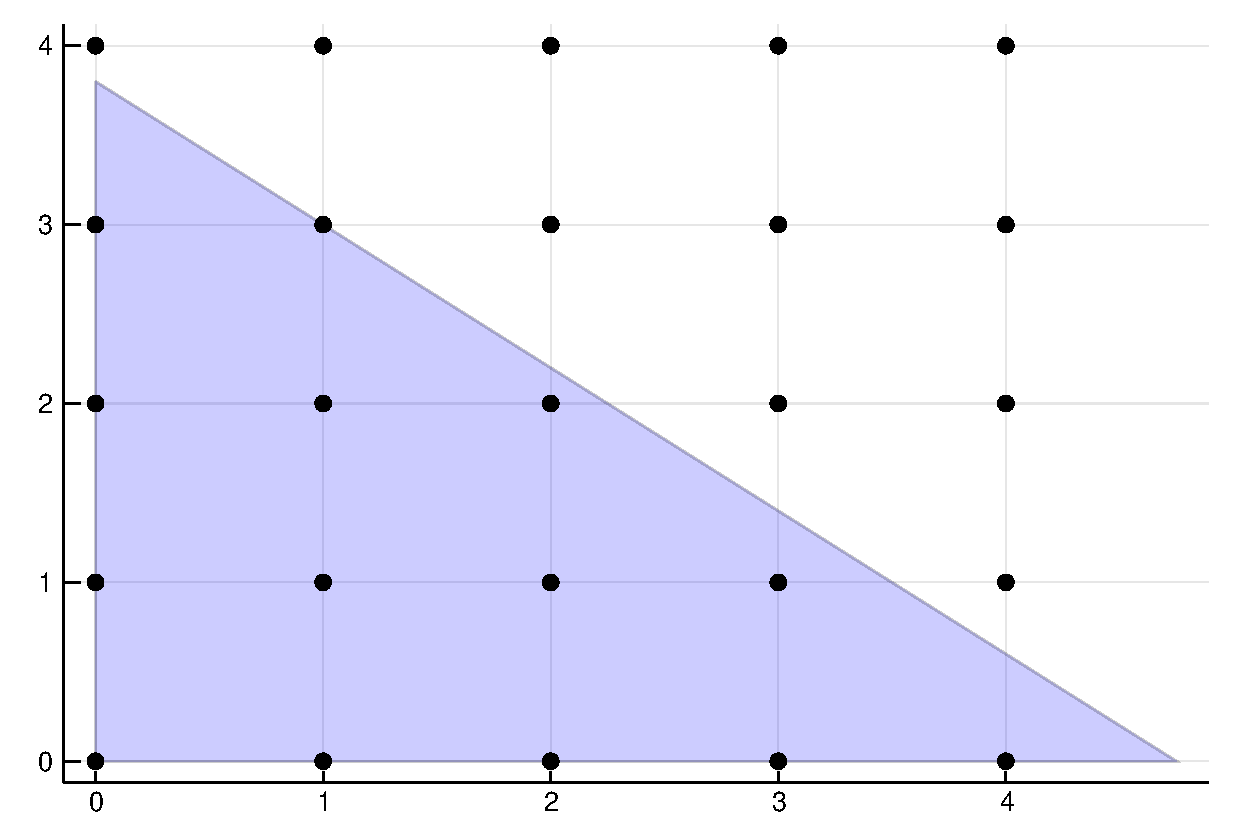
\includegraphics[scale = 0.4]{knapsack_fig.pdf}
\end{center}
where $P$ is the blue triangle and each integer point represents a pattern.  Feasible patterns lie inside the polytope $P$.  Note that we only need patterns that are maximal with respect to number of each type we cut.  Pictorially, we only need the patterns that are integer points represented as yellow dots in the picture below.
\begin{center}
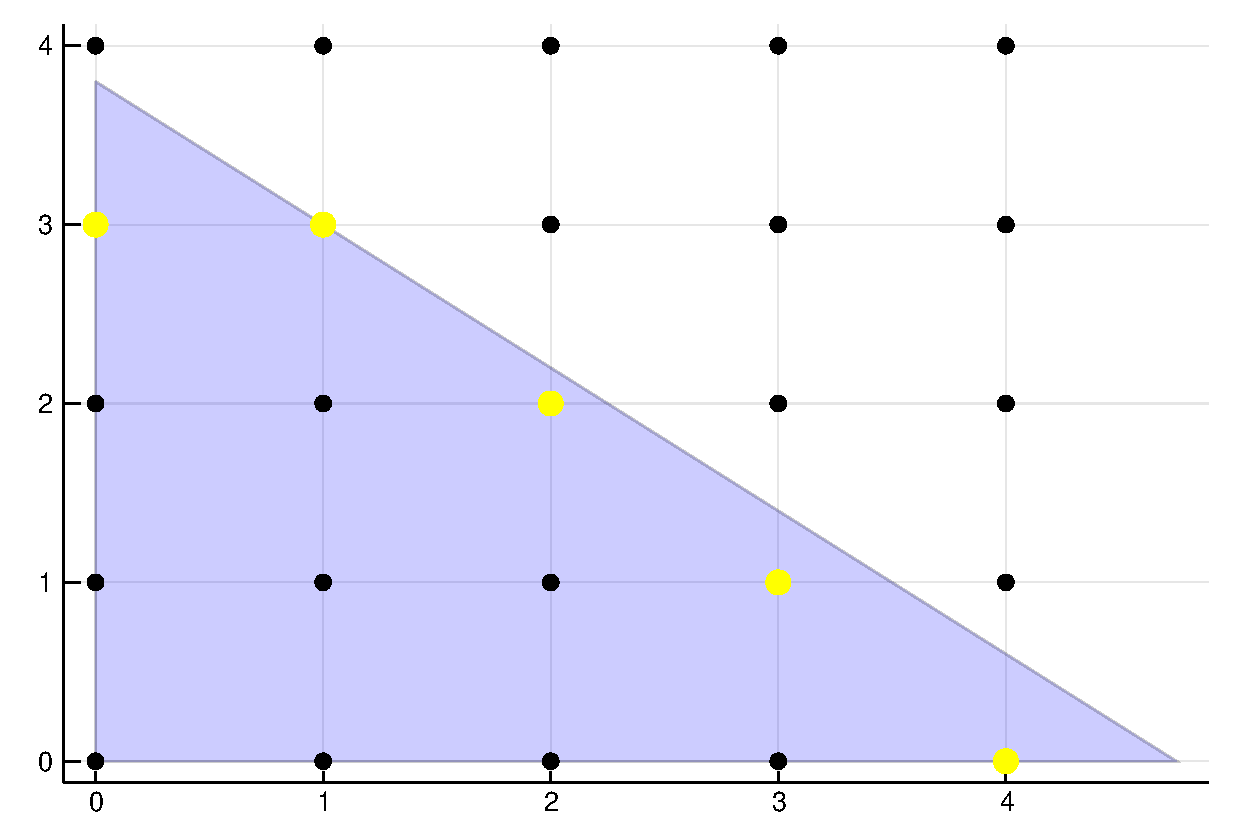
\includegraphics[scale = 0.4]{knapsack_fig_maximal.pdf}
\end{center}
For example, the pattern $[3,0,0]$ is not needed (only cut 3 of length 4m) since we could also use the patten $[4,0,0]$ (cut 4 of  length 4m) or we could even use the pattern $[3,1,0]$  (cut 3 of length 4m and 1 of length 5m).

%\begin{Verbatim}
%A = [ 0 0 1 0 2 1 2 3 4
%        0 1 0 2 1 2 2 1 0
%        3 2 2 1 1 0 0 0 0 ]
%\end{Verbatim}
% 



\subsection{Column Generation}
Consider the \eqref{LP:basis-solution}, but in this case we are instead minimizing.  Thus we can write it as 
 \begin{equation}
 \label{LP:basis-solution2}
\begin{split}
\min \quad & (c_N  - c_B B^{-1} N) x_N + c_B B^{-1} b  \\
\st  \quad &x_B +  B^{-1} N) x_N = B^{-1}b\\
& x \geq 0
\end{split}
\end{equation}
In our LP we have $c = \one$, that is, $c_i =1$ for all $i=1, \dots, k$.  Hence, we can write it as 
 \begin{equation}
 \label{LP:basis-solution3}
\begin{split}
\min \quad & (\one_N  - \one_B B^{-1} N) x_N + \one_B B^{-1} b  \\
\st  \quad &x_B +  B^{-1} N) x_N = B^{-1}b\\
& x \geq 0
\end{split}
\end{equation}
Now, if there exists a non-basic variable that could enter the basis and improve the objective, then there is one with a reduced cost that is negative.  For a particular non-basic variable, the coefficient on it is
\begin{equation}
\left( 1 -  \one_B B^{-1} N^i\right) x_i
\end{equation}
where $N^i$ is the $i$-th column of the matrix $N$.  Thus, we want to look for a column $a$ of $N$ such that 
\begin{equation}
1 -  \one_B B^{-1} a < 0 \ \  \Rightarrow \ \   1 < \one_B B^{-1} a
\end{equation}
\begin{general}{Pricing Problem}{(knapsack problem!)}
Given a current basis $B$ of the \emph{master} linear program, there exists a new column to add to the basis that improves the LP objective if and only if the following problem has an objective value strictly larger than 1
\begin{equation}
\begin{split}
\max\quad  &\one_B B^{-1} a\\
\st \quad & \sum_{i=1}^k L_i a_i \leq L\\
& a_i \in \Z_+ \text{ for } i=1, \dots, k
\end{split}
\end{equation}
\end{general}

\begin{example}{Pricing Problem}{(knapsack problem!)}
After choosing the initial columns .... 

we can find the objective function.... 


\begin{equation}
\begin{split}
\max\quad  & .......a\\
\st \quad & 4 a_1 + 5 a_2 + 6 a_3 \leq 19\\
& a_i \in \Z_+ \text{ for } i=1, \dots, k
\end{split}
\end{equation}
\end{example}
\subsection{Cutting Stock - Multiple widths}
Gurobi has as excellent demonstration application to look at:
\url{https://www.gurobi.com/cutting-stock-problem-with-multiple-master-rolls/}

\url{https://demos.gurobi.com/cutstock/}.




Here are some solutions:
\begin{itemize}
\item  \url{https://github.com/fzsun/cutstock-gurobi}.
\item \url{http://www.dcc.fc.up.pt/~jpp/mpa/cutstock.py}
\end{itemize}


Here is an AIMMS description of the problem:\\
\url{https://download.aimms.com/aimms/download/manuals/AIMMS3OM_CuttingStock.pdf}

% \beign{bmatrix} 1 \\ 1 \\ 1\end{bmatrix}


\section{Spanning Trees}
\label{sec:spanning-tree-models}

%\includegraphics[scale = 0.6]{minimum-weight-spanning-tree}
%~\cite{MARTIN1991119}
%
%
%\includegraphics[scale = 0.5]{minimum-spanning-tree-ip-model}
%
%\includegraphics[scale = 0.5]{minimum-spanning-tree-model-comparison}
%
%\includegraphics[scale = 0.5]{minimum-spanning-tree-list-of-models}
See~\cite{Abdelmaguid2018} for a list of 11 models for the minimum spanning tree and a comparison using CPLEX.


\section{Traveling Salesman Problem}
\label{sec:tsp-models}
See \url{http://www.math.uwaterloo.ca/tsp/index.html} for excellent material on the TSP.\\
See also this chapter \url{https://www.math.uwaterloo.ca/~bico/papers/comp_chapter1.pdf}.

Also, watch this excellent talk by Bill Cook "Postcards from the Edge of Possibility":
\url{https://m.youtube.com/watch?v=5VjphFYQKj8}

We consider a directed graph, graph $G = (N,A)$ of nodes $N$ and arcs $A$.   Arcs are directed edges.  Hence the arc $(i,j)$ is the directed path $i \to j$.

A \emph{tour}, or Hamiltonian cycle (see \refincludefigurestatic{wiki/File/William_Rowan_Hamilton_painting.jpg}), is a cycle that visits all the nodes in $N$ exactly once and returns back to the starting node.


Given costs $c_{ij}$ for each arc $(i,j) \in A$, the goal is to find a minimum cost tour.


\begin{general}{Traveling Salesman Problem}{\nphard}
Given a directed graph $G = (N,A)$ and costs $c_{ij}$ for all $(i,j) \in A$, find a tour of minimum cost.
\end{general}
\begin{center}
\textbf{ADD TSP FIGURE}
%\includegraphics[scale = 0.4]{tsp-solution}\footnotemark
\end{center}
In the figure, the nodes $N$ are the cities and the arcs $A$ are the directed paths $\text{city} i \to \text{city} j$.

\paragraph{Models}
When constructing an integer programming model for TSP, we define variables $x_{ij}$ for all $(i,j) \in A$ as 
$$
x_{ij } = 1 \text{ if the arc $(i,j)$ is used  and   }  x_{ij} = 0 \text{   otherwise.}
$$

We want the model to satisfy the fact that each node should have exactly one incoming arc and one leaving arc.  Furthermore, we want to prevent self loops.  Thus, we need the constraints:

\begin{align}
\label{eq:tsp-part-model}
\sum_{j\in N} x_{ij} &= 1 & \text{ for all } i \in N \ \ \text{ [outgoing arc]}\\
\sum_{i \in N} x_{ij} &= 1 & \text{ for all } j \in N \ \ \text{ [incoming arc]}\\
\label{eq:tsp-part-model3}
x_{ii} &= 0 & \text{ for all } i \in N \ \ \text{ [no self loops]} 
\end{align}

Unfortunately, these constraints are not enough to completely describe the problem.  The issue is that \emph{subtours} may arise.  For instance
\begin{center}
\textbf{ADD SUBTOURS FIGURE}
%\includegraphics[scale = 0.4]{tsp-subtours}\footnotemark
\end{center}
\subsubsection{MTZ Model}

\begin{itemize}
\item This model adds variables $u_i \in \Z$ with $1 \leq u_i \leq n$ that decide the order in which nodes are visited.
\item We set $u_1 = 1$ to set a starting place.
\item Crucially, this model relies on the following fact\\
\begin{center}
\emph{
Let  $x$ be a solution to \eqref{eq:tsp-part-model}-\eqref{eq:tsp-part-model3} with $x_{ij} \in \{0,1\}$.  If there exists a subtour in this solution that contains the node $1$, then there also exists a subtour that does not contain the node $1$.}
\end{center}
\end{itemize}

The following model adds constraints
\begin{equation}
\text{ If } x_{ij} = 1, \ \ \text{then} \ \ u_i + 1 \leq u_j.
\end{equation}
This if-then statement can be modeled with a big-M, choosing $M = n$ is a sufficient upper bound.  Thus, it can be written as 
\begin{equation}
\label{mtz-constraint}
u_i + 1 \leq u_j + n(1-x_{ij})
\end{equation}
Setting these constraints to be active enforces the order $u_i < u_j$.    

Consider a subtour now  $2 \to 5 \to 3 \to 2$.  Thus, $x_{25} = x_{53} = x_{32} = 1$.  Then using the constraints from \eqref{mtz-constraint}, we have that 
\begin{equation}
u_2 < u_5 < u_3 < u_2,
\end{equation}
but this is infeasible since we cannot have $u_2 < u_2$.  

As stated above, if there is a subtour containing the node $1$, then there is also a subtour not containing the node $1$.  Thus, we can enforce these constraints to only prevent subtours that don't contain the node $1$.  Thus, the full tour that contains the node $1$ will still be feasible.

This is summarized in the following model:
\begin{general}{Traveling Salesman Problem - MTZ Model}{}
\begin{align}
\min \sum_{i,j \in N} c_{ij} x_{ij}\\
\sum_{j\in N} x_{ij} &= 1 & \text{ for all } i \in N \ \ \text{ [outgoing arc]}\\
\sum_{i \in N} x_{ij} &= 1 & \text{ for all } j \in N \ \ \text{ [incoming arc]}\\
x_{ii} &= 0 & \text{ for all } i \in N \ \ \text{ [no self loops]} \\
u_i + 1 & \leq u_j + n(1-x_{ij})  & \text{ for all } i,j \in N, i,j \neq 1 \ \ \text{[prevents subtours]}\\
u_1 &= 1\\
2 \leq & u_i \leq n & \text{ for all } i \in N, i \neq 1\\
& u_i \in \Z & \text{ for all } i \in N\\
& x_{ij} \in \{0,1\} & \text{ for all } i,j \in N
\end{align}
\end{general}


\begin{example}{}{}

%\begin{center}
%\tikz[nodes={draw, circle}]
%\graph { subgraph K_n [n=4,clockwise,radius=3cm] };
%\end{center}
Distance Matrix:
\begin{verbatim}
A \ B | 1  2  3  4
----------------------
1     | 0  1  2  3
2     | 1  0  1  2
3     | 2  1  0  4
4     | 3  2  4  0
\end{verbatim}


\begin{align*}\min\quad & x_{1,2} + 2 x_{1,3} + 3 x_{1,4} + x_{2,1} + x_{2,3} + 2 x_{2,4} + \\ 2 x_{3,1} + x_{3,2} + 4 x_{3,4} + 3 x_{4,1} + 2 x_{4,2} + 4 x_{4,3}\\
\text{Subject to} \quad \\
 & x_{1,1} + x_{1,2} + x_{1,3} + x_{1,4} = 1& \text{ outgoing from node 1}\\
  & x_{2,1} + x_{2,2} + x_{2,3} + x_{2,4} = 1& \text{ outgoing from node 2}\\
 & x_{3,1} + x_{3,2} + x_{3,3} + x_{3,4} = 1& \text{ outgoing from node 3}\\
 & x_{4,1} + x_{4,2} + x_{4,3} + x_{4,4} = 1& \text{ outgoing from node 4}\\
 \\
  & x_{1,1} + x_{2,1} + x_{3,1} + x_{4,1} = 1& \text{ incoming to node 1}\\
 & x_{1,2} + x_{2,2} + x_{3,2} + x_{4,2} = 1& \text{ incoming to node 2}\\
 & x_{1,3} + x_{2,3} + x_{3,3} + x_{4,3} = 1& \text{ incoming to node 3}\\ 
 & x_{1,4} + x_{2,4} + x_{3,4} + x_{4,4} = 1& \text{ incoming to node 4}\\
 \\
 & x_{1,1} = 0 & \text{No self loop with node 1}\\
 & x_{2,2} = 0& \text{No self loop with node 2}\\
 & x_{3,3} = 0& \text{No self loop with node 3}\\
 & x_{4,4} = 0& \text{No self loop with node 4}\\
 \\
 & u_{1} = 1 & \text{Start at node 1}\\
  &2  \leq u_{i} \leq 4, \quad\forall i \in \{2,3,4\}\\
 & u_{2} +1 \leq  u_{3} + 4 (1-x_{2,3})\\
 & u_{2} +1 \leq u_{4} + 4 (1-x_{2,4}) \leq 3\\
 & u_{3} +1 \leq u_{2} + 4 (1-x_{3,2}) \leq 3\\
 & u_{3} +1 \leq u_{4} + 4 (1-x_{3,4}) \leq 3\\
 & u_{4} +1 \leq u_{2} + 4 (1-x_{4,2}) \leq 3\\
 & u_{4} +1 \leq u_{3} + 4 (1-x_{4,3}) \leq 3\\
 & x_{i,j} \in \{0,1\} \quad\forall i\in \{1,2,3,4\}, j \in \{1,2,3,4\}\\
 & u_{i} \in \mathbb{Z}, \quad\forall i \in \{1,2,3,4\}\\
\end{align*}
\end{example}


\begin{example}{5 nodes}

\begin{align*}\min\quad & x_{1,2} + 2 x_{1,3} + 3 x_{1,4} + 4 x_{1,5} + x_{2,1} + x_{2,3} + 2 x_{2,4} + 2 x_{2,5} + 2 x_{3,1} + \\&x_{3,2} + 4 x_{3,4} + x_{3,5} + 3 x_{4,1} + 2 x_{4,2} + 4 x_{4,3} + 2 x_{4,5} + \\&4 x_{5,1} + 2 x_{5,2} + x_{5,3} + 2 x_{5,4}\\
\text{Subject to} \quad  
 & x_{1,1} + x_{1,2} + x_{1,3} + x_{1,4} + x_{1,5} = 1\\
 & x_{2,1} + x_{2,2} + x_{2,3} + x_{2,4} + x_{2,5} = 1\\
 & x_{3,1} + x_{3,2} + x_{3,3} + x_{3,4} + x_{3,5} = 1\\
 & x_{4,1} + x_{4,2} + x_{4,3} + x_{4,4} + x_{4,5} = 1\\
 & x_{5,1} + x_{5,2} + x_{5,3} + x_{5,4} + x_{5,5} = 1\\
 \\
&x_{1,1} + x_{2,1} + x_{3,1} + x_{4,1} + x_{5,1} = 1\\
 & x_{1,2} + x_{2,2} + x_{3,2} + x_{4,2} + x_{5,2} = 1\\
 & x_{1,3} + x_{2,3} + x_{3,3} + x_{4,3} + x_{5,3} = 1\\
 & x_{1,4} + x_{2,4} + x_{3,4} + x_{4,4} + x_{5,4} = 1\\
 & x_{1,5} + x_{2,5} + x_{3,5} + x_{4,5} + x_{5,5} = 1\\
\\
 & x_{1,1} = 0\\
 & x_{2,2} = 0\\
 & x_{3,3} = 0\\
 & x_{4,4} = 0\\
 & x_{5,5} = 0\\
 \\
 & u_{1} = 1\\
 & 2 \leq u_{i} \leq 5 \quad\forall i \in \{1,2,3,4,5\}\\
 & u_{2} +1 \leq u_{3} + 5 (1-x_{2,3})\\
 & u_{2} +1 \leq u_{4} + 5  (1-x_{2,4})\\
  & u_{2} +1 \leq  u_{5} + 5 (1-x_{2,5} )\\
 & u_{3} +1 \leq u_{2} + 5  (1-x_{3,2})\\
 & u_{3} +1 \leq u_{4} + 5  (1-x_{3,4})\\
 & u_{4} +1 \leq u_{2} + 5  (1-x_{4,2})\\
 & u_{4} +1 \leq u_{3} + 5  (1-x_{4,3})\\
 & u_{3} +1 \leq  u_{5} + 5 (1-x_{3,5} )\\
 & u_{4} +1 \leq  u_{5} + 5 (1-x_{4,5})\\
 & u_{5} +1 \leq  u_{2} + 5 (1-x_{5,2} )\\
 & u_{5}+1 \leq  u_{3} + 5 (1-x_{5,3} )\\
 & u_{5} +1 \leq  u_{4} + 5 (1-x_{5,4} )\\
 & x_{i,j} \in \{0,1\} \quad\forall i \in \{1,2,3,4,5\}, j \in \{1,2,3,4,5\}\\
 & u_{i} \in \mathbb{Z}, \quad\forall i \in \{1,2,3,4,5\}
\end{align*}
\end{example}

\paragraph{Pros of this model}
\begin{itemize}
\item Small description
\item Easy to implement
\end{itemize}
\paragraph{Cons of this model}
\begin{itemize}
\item Linear relaxation is not very tight.  Thus, the solver may be slow when given this model.
\end{itemize}

\subsection{Dantzig-Fulkerson-Johnson Model}
This model does not add new variables.  Instead, it adds constraints that conflict with the subtours.  For instance, consider a subtour
\begin{equation}
2 \to 5 \to 3 \to 2.
\end{equation}
We can prevent this subtour by adding the constraint
\begin{equation}
x_{25} + x_{53} + x_{32}  \leq 2
\end{equation}
meaning that at most 2 of those arcs are allowed to happen at the same time.  In general, for any subtour $S$, we can have the \emph{subtour elimination constraint}
\begin{align}
\sum_{(i,j) \in S} x_{ij} &\leq |S| - 1  & \text{ Subtour Elimination Constraint}.
\end{align}
In the previous example with $S = \{(2,5), (5,3), (3,2)\}$ we have $|S| = 3$, where $|S|$ denotes the size of the set $S$.

This model suggests that we just add all of these subtour elimination constraints.

\begin{general}{Traveling Salesman Problem - DFJ Model}{}
\begin{align}
\label{eq:tsp-DFJ-model}
\min \sum_{i,j \in N} c_{ij} x_{ij}\\
\sum_{j\in N} x_{ij} &= 1 & \text{ for all } i \in N \ \ \text{ [outgoing arc]}\\
\sum_{i \in N} x_{ij} &= 1 & \text{ for all } j \in N \ \ \text{ [incoming arc]}\\
x_{ii} &= 0 & \text{ for all } i \in N \ \ \text{ [no self loops]} \\
\sum_{(i,j) \in S} x_{ij} &\leq |S| -1  & \text{ for all subtours } S \ \ \text{[prevents subtours]}\\
& x_{ij} \in \{0,1\} & \text{ for all } i,j \in N
\end{align}
\end{general}

%\begin{tikzpicture}
%
%\tikzset{vertex/.style = {shape=circle,draw,minimum size=1.5em}}
%\tikzset{edge/.style = {->,> = latex'}}
%% vertices
%\node[vertex] (a) at  (0,0) {};
%\node[vertex] (b) at  (4,3) {};
%\node[vertex] (c) at  (8,0) {};
%\node[vertex] (d) at  (4,-3) {$t$};
%\node[vertex] (a1) at (1.5,0) {};
%\node[vertex] (a2) at (3,0) {};
%%edges
%\draw[edge] (b) to (a);
%\draw[edge] (b) to (c);
%\draw[edge] (a) to (d);
%\draw[edge] (c) to (d);
%
%\draw[edge] (a)  to[bend left] (a1);
%\draw[edge] (a1) to[bend left] (a);
%
%\draw[edge] (a1) to[bend left] (a2);
%\draw[edge] (a2) to[bend left] (a1);
%
%\path (a2) to node {\dots} (c);
%\node [shape=circle,minimum size=1.5em] (a3) at (4.5,0) {};
%\draw[edge] (a2) to[bend left] (a3);
%\draw[edge] (a3) to[bend left] (a2);
%
%\node [shape=circle,minimum size=1.5em] (c1) at (6.5,0) {};
%\draw[edge] (c) to[bend left] (c1);
%\draw[edge] (c1) to[bend left] (c);
%\end{tikzpicture}


\begin{example}{DFJ Model for $n=4$ nodes}{}


%\begin{center}
%\tikz[nodes={draw, circle}]
%\graph { subgraph K_n [n=4,clockwise,radius=3cm] };
%\end{center}
Distance Matrix:
\begin{verbatim}
A \ B | 1  2  3  4
----------------------
1     | 0  1  2  3
2     | 1  0  1  2
3     | 2  1  0  4
4     | 3  2  4  0
\end{verbatim}


%\begin{align}\min\quad & x_{1,2} + 2 x_{1,3} + 3 x_{1,4} + x_{2,1} + x_{2,3} + 2 x_{2,4} + 2 x_{3,1} + x_{3,2} + 4 x_{3,4} + 3 x_{4,1} + 2 x_{4,2} + 4 x_{4,3}\\
%\text{Subject to} \quad & x_{1,1} + x_{2,1} + x_{3,1} + x_{4,1} = 1\\
% & x_{1,2} + x_{2,2} + x_{3,2} + x_{4,2} = 1\\
% & x_{1,3} + x_{2,3} + x_{3,3} + x_{4,3} = 1\\
% & x_{1,4} + x_{2,4} + x_{3,4} + x_{4,4} = 1\\
% & x_{1,1} + x_{1,2} + x_{1,3} + x_{1,4} = 1\\
% & x_{2,1} + x_{2,2} + x_{2,3} + x_{2,4} = 1\\
% & x_{3,1} + x_{3,2} + x_{3,3} + x_{3,4} = 1\\
% & x_{4,1} + x_{4,2} + x_{4,3} + x_{4,4} = 1\\
% & x_{1,1} = 0\\
% & x_{2,2} = 0\\
% & x_{3,3} = 0\\
% & x_{4,4} = 0\\
% & x_{i,j} \in \{0,1\} \quad\forall i \in \{1,2,3,4\}, j \in \{1,2,3,4\}\\
%\end{align}


\begin{align*}{1}\min\quad & x_{1,2} + 2 x_{1,3} + 3 x_{1,4} + x_{2,1} + x_{2,3} + 2 x_{2,4} \\& + 2 x_{3,1} + x_{3,2} + 4 x_{3,4} + 3 x_{4,1} + 2 x_{4,2} + 4 x_{4,3}\\
\\
\text{Subject to} \quad \\
 & x_{1,1} + x_{1,2} + x_{1,3} + x_{1,4} = 1& \text{ outgoing from node 1}\\
  & x_{2,1} + x_{2,2} + x_{2,3} + x_{2,4} = 1& \text{ outgoing from node 2}\\
 & x_{3,1} + x_{3,2} + x_{3,3} + x_{3,4} = 1& \text{ outgoing from node 3}\\
 & x_{4,1} + x_{4,2} + x_{4,3} + x_{4,4} = 1& \text{ outgoing from node 4}\\
 \\
  & x_{1,1} + x_{2,1} + x_{3,1} + x_{4,1} = 1& \text{ incoming to node 1}\\
 & x_{1,2} + x_{2,2} + x_{3,2} + x_{4,2} = 1& \text{ incoming to node 2}\\
 & x_{1,3} + x_{2,3} + x_{3,3} + x_{4,3} = 1& \text{ incoming to node 3}\\ 
 & x_{1,4} + x_{2,4} + x_{3,4} + x_{4,4} = 1& \text{ incoming to node 4}\\
 \\
 & x_{1,1} = 0 & \text{No self loop with node 1}\\
 & x_{2,2} = 0& \text{No self loop with node 2}\\
 & x_{3,3} = 0& \text{No self loop with node 3}\\
 & x_{4,4} = 0& \text{No self loop with node 4}\\
 \\
 & x_{1,2} + x_{2,1} \leq 1& S = [(1,2), (2,1)]\\
 & x_{1,3} + x_{3,1} \leq 1& S = [(1,3), (3,1)]\\
 & x_{1,4} + x_{4,1} \leq 1& S = [(1,4), (4,1)]\\
 & x_{2,3} + x_{3,2} \leq 1& S = [(2,3), (3,2)]\\
 & x_{2,4} + x_{4,2} \leq 1& S = [(2,4), (4,2)]\\
 & x_{3,4} + x_{4,3} \leq 1& S = [(3,4), (4,3)]\\
 & x_{2,1} + x_{1,3} + x_{3,2} \leq 2 & S = [(2,1), (1,3), (3,2)]\\
 & x_{1,2} + x_{2,3} + x_{3,1} \leq 2& S = [(1,2), (2,3), (3,1)]\\
 & x_{3,1} + x_{1,4} + x_{4,3} \leq 2& S = [(3,1), (1,4), (4,3))]\\
 & x_{1,3} + x_{3,4} + x_{4,1} \leq 2& S = [(1,3),(3,4), (4,1)]\\
 & x_{2,1} + x_{1,4} + x_{4,2} \leq 2& S = [(2,1), (1,4), (4,2)]\\
 & x_{1,2} + x_{2,4} + x_{4,1} \leq 2& S = [(1,2), (2,4), (4,1)]\\
 & x_{3,2} + x_{2,4} + x_{4,3} \leq 2& S = [(3,2), (2,4), (4,3)]\\
 & x_{2,3} + x_{3,4} + x_{4,2} \leq 2& S = [(2,3), (3,4), (4,2)]\\
 \\
 & x_{i,j} \in \{0,1\} \quad\forall i \in \{1,2,3,4\}, j \in \{1,2,3,4\}\\
\end{align*}
%\includegraphics[scale = 0.5]{CompleteGraph4Nodes}



%\includegraphics[scale = 0.5]{CompleteGraphCycles4-850}\footnotemark
%\footnotetext{\url{http://mathworld.wolfram.com/CompleteGraph.html}}

\end{example}


\begin{example}{}{}

Consider a graph on 5 nodes.

%\begin{center}
%\tikz[nodes={draw, circle}]
%\graph { subgraph K_n [n=5,clockwise,radius=3cm] };
%\end{center}

Here are all the subtours of length at least 3 and also including the full length tours.


Hence, there are many subtours to consider.
\end{example}


\paragraph{Pros of this model}
\begin{itemize}
\item Very tight linear relaxation
\end{itemize}
\paragraph{Cons of this model}
\begin{itemize}
\item Exponentially many subtours $S$ possible, hence this model is too large to write down.
\end{itemize}

\paragraph{Solution: Add subtour elimination constraints as needed.  We will discuss this in a future section on \emph{cutting planes}}.

\subsection{Traveling Salesman Problem - Branching Solution}
We will see in the next section
\begin{enumerate}
\item That the constraint \eqref{eq:tsp-part-model}-\eqref{eq:tsp-part-model3}  always produce integer solutions as solutions to the linear relaxation.
\item A way to use branch and bound (the topic of the next section) in order to avoid subtours.
\end{enumerate}


\section{Google maps data}
\url{https://www.geeksforgeeks.org/python-calculate-distance-duration-two-places-using-google-distance-matrix-api/}



\section{Literature}

Gilmore-Gomory Cutting Stock~\cite{Gilmore-Gomory}

\url{http://www.optimization-online.org/DB_HTML/2018/06/6648.html}

\url{http://www.optimization-online.org/DB_HTML/2018/06/6670.html}

\url{http://www.optimization-online.org/DB_FILE/2017/11/6331.pdf}

\end{document}
